%!TEX root = ../CallenThermo.tex
%----------------------------------------------------------------------------------------
%	翻译:SI, 哪托儿闹海
%   校对:lh, SI
%----------------------------------------------------------------------------------------


\chapter{形式关系与样例系统}
\label{chap3}

\section{热力学Euler方程}
\label{sec3.1}
上一章从基本假设出发解出了平衡态条件,下面深入探究基本方程的数学特征。

基本方程的一阶齐次性使得它可以写成更方便的形式,称为Euler形式。

从一阶齐次性的定义出发,对任意常数$\lambda$都有:
\begin{equation}
\label{equ3.1}
    U(\lambda S, \lambda X_1, \dots, \lambda X_t) = \lambda U(S, X_1, \dots, X_t).
\end{equation}
等式两侧对$\lambda$求导:
\begin{align}
    \frac{ \partial U(\dots, \lambda X_k, \dots)}{\partial (\lambda S)} \frac{\partial (\lambda S)}{\partial \lambda} + \frac{ \partial U(\dots, \lambda X_k, \dots)}{\partial (\lambda X_j)} \frac{\partial (\lambda X_j)}{\partial \lambda} \notag \\
    + \dots = U(S, X_1, \dots, X_t) \label{equ3.2} \\
    \frac{\partial U(\dots, \lambda X_k, \dots)}{\partial (\lambda S)} S + \sum_{j = 1}^t \frac{\partial U(\dots, \lambda X_k, \dots)}{\partial (\lambda X_j)} X_j \notag \\
    = U(S, X_1, \dots, X_t) \label{equ3.3}
\end{align}
方程对任意$\lambda$都成立,取$\lambda = 1$可得:
\begin{align}
    \pUpS S + \sum_{j = 1}^t \frac{\partial U}{\partial X_j} X_j + \dots = U \label{equ3.4} \\
    U = TS + \sum_{j = 1}^t P_j X_j \label{equ3.5}
\end{align}
对于简单系统,上式写为
\begin{equation}
\label{equ3.6}
    U = TS - PV + \mu_1 N_1 + \dots + \mu_r N_r
\end{equation}
\eqref{equ3.5}或\eqref{equ3.6}式是齐次函数Euler定理\mpar{若函数$f(x, y, \dots)$满足$f(\lambda x, \lambda y, \dots) = \lambda^n f(x, y, \dots)$, 则$f$称为$n$阶齐次的。齐次函数Euler定理为$x \frac{\partial f}{\partial x} + y \frac{\partial f}{\partial y} + \dots = n f$.}的一阶齐次情形在热力学理论的应用。公式的推导过程即为齐次定理的证明过程。\eqref{equ3.5}或\eqref{equ3.6}式称为(热力学)Euler关系。

类似地,熵表象下Euler关系的形式为
\begin{align}
    S &= \sum_{j = 0}^t F_j X_j \label{equ3.7} \\
    S &= \left(\frac{1}{T} \right) U + \left( \frac{P}{T} \right) V - \sum_{k = 1}^r \left( \frac{\mu_k}{T} \right) N_k. \label{equ3.8}
\end{align}

\subsection*{习题}
\begin{itemize}
\item[3.1-1.] 写出习题1.10-1当中具有物理意义的基本方程的Euler形式。
\end{itemize}

\section{Gibbs-Duhem关系}
\label{sec3.2}
第二章导出了用温度、压强和化学势表示的平衡条件。这些强度量的引入过程比较相似,事实上,它们的形式体系也是对称的。尽管号称有对称性,但我们对温度与压强有着非常直观的感受,而对化学势就差了一点。有趣的是,这些强度量之间不是完全独立的,它们之间存在函数关系,例如单组分系统的化学势$\mu$可表示为$T, P$的函数。

这种关系是基本方程一阶齐次性的结果。考虑某一单组分系统,基本方程可写为$u = u(s, v)$(即\eqref{equ2.19}式);三个强度量也都是$s, v$的函数,原则上这三个状态方程
\begin{align*}
    T &= T(u, v) \\
    P &= P(u, v) \\
    \mu &= \mu (u, v)
\end{align*}
可消去$u, v$形成一个关于$T, P, \mu$的方程。

容易推广到一般情况,关键还是数清楚变量与方程的数目。设基本方程具有$t + 1$个广延量:
\begin{equation}
\label{equ3.9}
    U = U(S, X_1, X_2, \dots, X_t).
\end{equation}
由此产生$t + 1$个状态方程:
\begin{equation}
\label{equ3.10}
    P_k = P_k(S, X_1, X_2, \dots, X_t).
\end{equation}
令\eqref{equ2.14}式中的任意参量$\lambda$为$\lambda = 1 / X_t$,可得
\begin{equation}
\label{equ3.11}
	P_k = P_k \left( \frac{S}{X_t}, \frac{X_1}{X_t}, \dots, \frac{X_{t-1}}{X_t}, 1 \right).
\end{equation}
可见这$t + 1$个强度量都是关于$t$个变量的函数,从$t + 1$个方程中消去$t$个变量就得到强度量之间的关系。

知道基本方程的具体形式就能求出强度量之间关系的具体形式。给定基本方程之后的套路即为$\eqref{equ3.9} \sim \eqref{equ3.11}$式的过程。

这种关系的微分形式(称为{\bf Gibbs-Duhem关系})可以从Euler关系直接导出。对\eqref{equ3.5}式微分得到
\begin{equation}
\label{equ3.12}
	\,\mathrm dU = T\,\mathrm dS + S\,\mathrm dT + \sum_{j = 1}^t P_j \,\mathrm dX_j + \sum_{j = 1}^t X_j \,\mathrm dP_j.
\end{equation}
由\eqref{equ2.6}式可得
\begin{equation}
\label{equ3.13}
	\,\mathrm dU = T\,\mathrm dS + \sum_{j = 1}^t P_j \,\mathrm dX_j.
\end{equation}
以上两式相减即得到Gibbs-Duhem关系:
\begin{equation}
\label{equ3.14}
	S\,\mathrm dT + \sum_{j = 1}^t X_j \,\mathrm dP_j = 0.
\end{equation}
对于单组分简单系统有
\begin{equation}
\label{equ3.15}
	S\,\mathrm dT - V\,\mathrm dP + N\,\mathrm d\mu = 0.
\end{equation}
或者
\begin{equation}
\label{equ3.16}
	\,\mathrm d\mu = -s\,\mathrm dT + v\,\mathrm dP
\end{equation}
可见化学势的变化与温度及压强的变化有关,而非独立变化,并且$\mu, T, P$三者中已知任何两个的变化就能确定其余一个的变化。

Gibbs-Duhem关系是强度量之间关系的微分形式,将该式积分即得到显式形式,这是除$\eqref{equ3.9} \sim \eqref{equ3.11}$式外的另一种计算套路。Gibbs-Duhem关系的积分:
\[
	\int S(T, P_1, \dots, P_t) \,\rd T + \sum_{j = 1}^t \int X_j(T, P_1, \dots, P_t) \,\rd P_j = 0
\]
需要知道各广延量$X_j$用强度量$P_j$表示的形式,这可以从状态方程\mpar{状态方程:强度量作为广延量的函数}解出。因此积分Gibbs-Duhem关系必须知道系统的状态方程。

系统可独立变化的强度量个数称为系统的{\it 热力学自由度 (thermodynamic degrees of freedom)}。{\it 一个具有$r$种组分的简单系统的热力学自由度为$r + 1$.}

熵表象下的Gibbs-Duhem关系依旧表示为全体广延量与相应强度量微分之积的和为零:
\begin{align}
	&\sum_{j = 0}^t X_j \,\mathrm dF_j = 0 \label{equ3.17} \\
	&U \,\mathrm d\left( \frac{1}{T} \right) + V \,\mathrm d\left( \frac{P}{T} \right) - \sum_{k = 1}^r N_k \,\mathrm d\left( \frac{\mu_k}{T}\right) = 0 \label{equ3.18}
\end{align}


\subsection*{习题}
\begin{itemize}
\item[3.2-1.] 某系统的基本方程为
\[
	U = \left( \frac{v_0^2 \theta}{R^3} \right) \frac{S^4}{NV^2}
\]
求$T, P, \mu$之间的函数关系。
\end{itemize}

\section{形式关系总结}
\label{sec3.3}
现在总结一下能量表象的热力学体系结构。简明起见,考虑单组分的简单系统,它的基本方程
\begin{equation}
\label{equ3.19}
    U = U(S, V, N)
\end{equation}
包含了该系统所有的热力学信息。定义了温度$T \equiv \partial U / \partial S$等强度量之后,从基本方程可以导出三个状态方程:
\begin{align}
    T &= T(S, V, N) = T(s, v) \label{equ3.20} \\
    P &= P(S, V, N) = S(s, v) \label{equ3.21} \\
    \mu &= \mu(S, V, N) = \mu(s, v) \label{equ3.22}
\end{align}
如果三个状态方程{\it 均}已知,将它们带入Euler关系,即可重新得到基本方程。{\it 因此三个状态方程整体等价于基本方程,}二者都蕴含系统的全部热力学信息,单个的状态方程的热力学信息量少于基本方程。

如果已知两个状态方程,带入Gibbs-Duhem关系再积分即可得到第三个,只是这样得到的状态方程含有一个未定的积分常数。因此两个状态方程(几乎)能够确定基本方程,只差一个未定常数。

当已知两个状态方程时,推导基本方程有更直接、更便利的方法(当然,该方法与利用Gibbs-Duhem关系的途径在逻辑上是等价的):直接积分单位摩尔数的热力学关系:
\begin{equation}
    \,\mathrm du = T\,\mathrm ds - P\,\mathrm dv.
\label{equ3.23}
\end{equation}
将已知的两个状态方程$T = T(s, v), P = P(s, v)$带入上式,即得到$u, s, v$之间的微分方程,再积分就得到
\begin{equation}
    u = u(s, v).
\label{equ3.24}
\end{equation}
这正是基本方程。当然,这个方程里有一个未定的积分常数。

内能总可以表为除了$S, V, N$以外的其它参量的函数。例如$U = U(S, V, N)$与$T = T(S, V, N)$联立消去$S$得到方程$U = U(T, V, N)$. 不过,必须强调的是,这样的方程{\it 并非}基本方程,不包含全部热力学信息。比如,在考虑到$T \equiv \partial U / \partial S$之后,$U = U(T, V, N)$实际上是个偏微分方程。即使它可积,积出的基本方程也带有未定函数。

如果基本方程$U = U(S, V, N)$已知,则相应的$U = U(T, V, N)$唯一确定;但反之不然,确定的$U = U(T, V, N)$并不唯一对应$U = U(S, V, N)$. 它们携带着的都是正确的信息. $U = U(S, V, N)$与$U = U(T, V, N)$都是正确的,但只有前者含有最完整的信息。  

上述内容可以用如下的图例简单说明。设$V, N$不变,内能$U$只随$S$变化,相应的$U\text{-}S$函数图像如图3.1(a)中的实线,这条曲线唯一确定了图3.1(b)所示的$U\text{-}T$曲线,因为$U(S)$每一点都有确定的斜率$T \equiv \partial U / \partial S$, 从而决定了$U(T)$。但如果反过来,已知$U(T)$函数(亦即,一个状态方程),能否决定$U(S)$? 当然不能。 图3.1(a)中的每条虚线之间之差一个“平移”\mpar{这来自求解偏微分方程$U = U(\partial U / \partial S)$留下的“积分常数”。},它们在相同的$U$处的斜率相等,{\it 都能}导出给定的$U(T)$。因此,图3.1(a)可以导出3.1(b),反之则不然。等价的说法是,只有$U = U(S)$才是基本关系。接下来在讨论几个特定的热力学样例系统后,我们将建立正式的理论结构。

{
	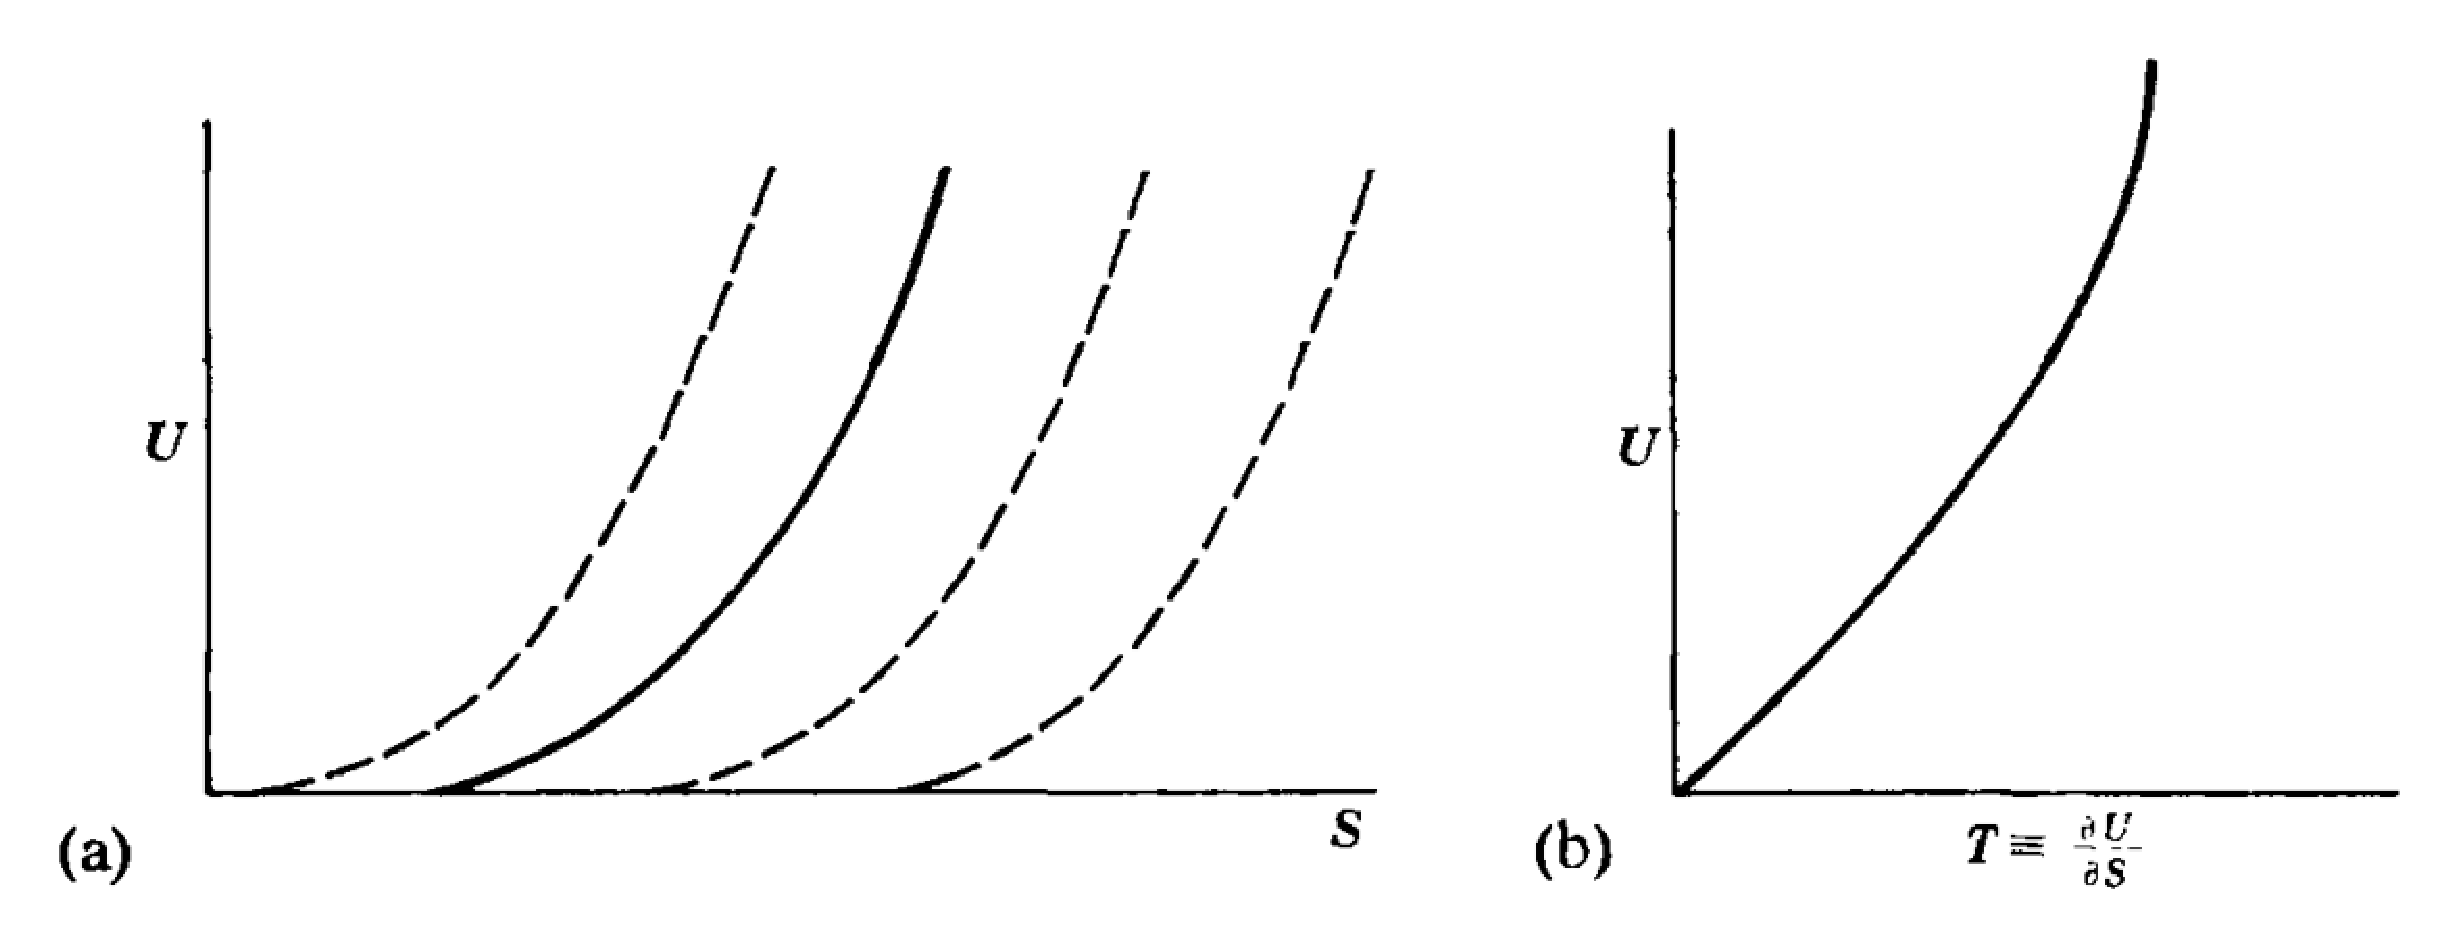
\includegraphics[scale=0.25]{fig3_1.eps} 
	\figcaption{ }
}

\begin{example}

某热力学系统满足条件
\begin{align*}
    U &= \frac{1}{2} PV, \\
    T^2 &= \frac{AU^{3/2}}{VN^{1/2}}.
\end{align*}
其中$A$是大于零的常数。求系统的基本方程。

{\bf 解}

已知条件中出现的独立变量为$U, V, N$,因此采用熵表象求解,首先将这两个已知方程化为熵表象标准形式:
\begin{align*}
    \frac{1}{T} &= A^{-1/2} u^{-3/4} v^{1/2} \\
    \frac{P}{T} &= 2A^{-1/2} u^{1/4} v^{-1/2}
\end{align*}
单位摩尔数基本方程的微分形式(类比\eqref{equ3.23}式)为
\begin{align*}
    ds &= \frac{1}{T} du + \frac{P}{T} dv \\
    &= A^{-1/2} (u^{-3/4} v^{1/2} du + 2u^{1/4} v^{-1/2} dv) \\
    &= 4A^{-1/2} d(u^{1/4} v^{1/2})
\end{align*}
解得
\begin{align*}
    s &= 4A^{-1/2} u^{1/4} v^{1/2} + s_0 \\
    \to S &= 4A^{-1/2} U^{1/4} V^{1/2} N^{1/4} + Ns_0
\end{align*}
当然还有另一种做法:首先对Gibbs-Duhem关系积分从而得到$\mu (u, v)$,然后将所得的三个状态方程带入Euler方程。读者应该尝试一下。

读者还应该注意例题中积分$ds$得到$s$的过程。$ds$关于$du$与$dv$的等式是一个{\it 偏微分方程},它{\it 不能}逐项积分,也不能用求解常微分方程的常用套路。我们通过“观察”对该方程进行积分,“恰好”发现$u^{-3/4} v^{1/2} du + 2u^{1/4} v^{-1/2} dv$正是$d(u^{1/4} v^{1/2})$. \sout{所以老师都不太愿意编习题}

\end{example}

\subsection*{习题}


\section{单组分/多组分简单理想气体}
\label{sec3.4}

单一组分简单理想气体可以用两个方程来描述:
\begin{align}
PV=NRT \label{equ3.25}\\
U=cNRT \label{equ3.26}
\end{align}
其中$c$是常值,$R$是一个普适的气体常数——热力学常数($R=N_Ak_B=8.3144\ \text{J/mole K}$).

上面的是比较理想化的方程。在现实世界中,人们发现,单原子气体(比如Ar、He)有可能符合方程\eqref{equ3.25}\eqref{equ3.26},如果其温度和压力再满足一定要求的话,具体而言,就是$k_BT$相较于电子激发能而言很小(比如当$T\lesssim \SI{e4}{\kelvin}$)而且压强相对较低,那么该气体就会符合上面的两个方程.此外,对所有的这种单原子气体都有$c=\frac{3}{2}$.

在一些更苛刻的条件下,其他的真实气体也有可能满足简单理想气体方程\eqref{equ3.25}\eqref{equ3.26},但是其$c$有可能不再是$3\over2$. 举个例子,双原子气体(比如NO、O$_2$)的$c$在一个很大的温度范围内约为${5\over2}$,在更高的温度下其$c$约为$7\over2$(两种情况的分界温度数量级一般在$10^3K$)。

通过方程\eqref{equ3.25}\eqref{equ3.26}可以确定基本方程. 方程\eqref{equ3.26}中内能$U$的形式很简单,这就启示我们:在熵表象下处理问题可能会更简单。将方程重写为合适的形式:
\begin{align}
\frac{1}{T}=cR\left(\frac{N}{U}\right)=\frac{cR}{u}\label{equ3.27}\\
\frac{P}{T}=R\left(\frac{N}{V}\right)=\frac{R}{v}\label{equ3.28}
\end{align}

如果将这两个熵状态方程代入Gibbs-Duhem关系式并积分,我们应该能得到第三个状态方程
\begin{equation}
\label{equ3.29}
\frac{\mu}{T}=u,v\text{的函数}
\end{equation}
Gibbs-Duhem关系式是:
\begin{equation}
\label{equ3.30}
\,\text{d}\left(\frac{\mu}{T}\right)=u\,\text{d}\left(\frac{1}{T}\right)+v\,\text{d}\left(\frac{P}{T}\right)
\end{equation}
最后这三个状态方程会被代入Euler方程,Euler方程为:
\begin{equation}
\label{equ3.31}
S = \left( \frac{1}{T} \right) U + \left( \frac{P}{T} \right) V - \frac{\mu}{T} N
\end{equation}

现在我们来实打实地干一番:将\eqref{equ3.25}\eqref{equ3.26}代入Gibbs-Duhem关系式可得:
\begin{equation}
\label{equ3.32}
\,\text{d}\left(\frac{\mu}{T}\right)=\mu\times\left(-\frac{cR}{u^2}\right)\,\text{d}u+v\times\left(-\frac{R}{v^2}\right)\,\text{d}v=-cR\frac{\text{d}u}{u}-R\frac{\text{d}v}{v}
\end{equation}
积分之后得
\begin{equation}
\label{equ3.33}
\frac{\mu}{T}- \left( \frac{\mu}{T} \right)_0 = -cR\ln{\frac{u}{u_0}}-R\ln{\frac{v}{v_0}}
\end{equation}
其中$u_0,v_0$是一个固定的参考态,$\displaystyle{ \left( \frac{\mu}{T} \right)_0 }$即随之产生的积分常数. 然后由Euler方程\eqref{equ3.31}可得
\begin{equation}
\label{equ3.34}
S=Ns_0+NR\ln\left[\left(\frac{U}{U_0}\right)^c\left(\frac{V}{V_0}\right)\left(\frac{N}{N_0}\right)^{-(c+1)}\right]
\end{equation}
其中
\begin{equation}
\label{equ3.35}
s_0=(c+1)R-\left(\frac{\mu_0}{T_0}\right)
\end{equation}
方程\eqref{equ3.34}就是要求的基本方程;如果积分常数$s_0$已知,那么方程\eqref{equ3.34}就包含了简单理想气体所有的热力学信息.

这种方式并非唯一的求解办法,甚至也非最常用的. 更直接的办法是将下式(摩尔量方程, molar equation)积分
\begin{equation}
\label{equ3.36}
\text{d}s=\left(\frac{1}{T}\right)\,\text{d}u+\left(\frac{P}{T}\right)\,\text{d}v
\end{equation}
在目前的问题中(理想气体),它变为
\begin{equation}
\label{equ3.37}
\text{d}s=c\left(\frac{R}{u}\right)\,\text{d}u+\left(\frac{R}{v}\right)\,\text{d}v
\end{equation}
积分后得
\begin{equation}
\label{equ3.38}
s = s_0 + cR \ln \left( \frac{u}{u_0} \right) + R\ln \left( \frac{v}{v_0} \right)
\end{equation}
这个方程与\eqref{equ3.34}等价.

应当注意,方程\eqref{equ3.37}是逐项可积的,但例3会提到,这样的方法在更一般的情况下无法实现. 方程\eqref{equ3.37}中,独立变量$u,v$的分离是一种巧合,这完全是由理想气体方程的特殊性所致. 这种特殊性使得方程\eqref{equ3.37}可以逐项积分.

两种或多种简单理想气体的混合物——“多组分简单理想气体”——可以由一个基本方程描述. 为了使形式更加简单,基本方程写成了参数形式,其中温度$T$作为参数。
\begin{equation}
\label{equ3.39}
\begin{split}
    S &= \sum_j N_j s_{j0} + \left(\sum_j N_jc_j\right) R \ln \frac{T}{T_0} + \sum_j N_jR\ln\left(\frac{V}{N_jv_0}\right) \\
    U &= \left(\sum_jN_jc_j\right)RT
\end{split}
\end{equation}
将$T$从这两个方程中消去,就得到一个具有标准形式$S=S(U,V,N_1,N_2,\cdots)$的方程.

观察\eqref{equ3.39}中关于某一种理想气体的项,并与该气体单独存在时的熵表达式作比较,可以发现如下事实(通常称作Gibbs定理):{\it 理想气体混合物的熵是其中每一种气体在温度为$T$下、单独占据体积$V$时的熵之和. }这个定理对所有的理想气体都成立(见第13章).

有趣的是,如果将方程\eqref{equ3.39}写成如下形式:
\begin{equation}
\label{equ3.40}
S=\sum_jN_js_{j0}+\left(\sum_jN_jc_{j}\right)R\ln{\frac{T}{T_0}}+NR\ln{\frac{V}{Nv_0}}-R\sum_jN_j\ln{\frac{N_j}{N}}
\end{equation}
则最后一项可视作“混合熵”.{\it 这一项代表了在同一温度和同一分子数密度$N_j/V_j = N/V$ (因此压强也相同)下,诸多分开的单一组分气体的熵之和与混合气体的熵之间的差异},见问题3.4-15. 上面这种阐述与Gibbs定理之间既有相当的差别,也有相似之处,读者应当仔细分辨. 混合熵可应用在分离同位素的问题上,我们将在\ref{sec4.4}节(例4)中进行阐述.

一个简单的“思想实验”就能简洁地证明Gibbs定理. 某圆柱体(图\ref{fig3.2})体积为$2V_0$,用3个隔板将其分成4个小室(分别用$\alpha,\beta,\gamma,\delta$来记),其中一个隔板固定在圆柱中间,两个可滑动的隔板在中心两边. 两边的两个隔板被链在一起,以保证它们之间的距离恒为圆柱长的一半(因此$V_\alpha=V_\gamma, V_\beta=V_\delta$). 最开始,两个滑动隔板分别在圆柱左边和圆柱中心,因此$V_\alpha=V_\gamma=0$. 此时小室$\beta$体积为$V_0$,其中充有$N_0$  mole理想气体A和$N_0$ mole的理想气体B的混合物. 而且小室$\delta$是真空的,整个系统的温度为$T$.

\begin{figure}
\centering
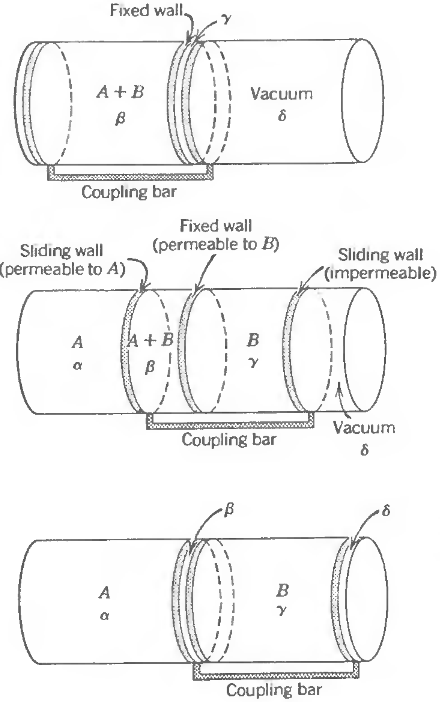
\includegraphics[width=.5\textwidth]{Pictures/fig3.2.png}
\figcaption{分离混合理想气体,用以证明 Gibbs 定理。}
\label{fig3.2}
\end{figure}

左边的滑动隔板可以任由气体A通过,但无法通过气体B,中间的固定隔板可任由气体B通过,但无法通过气体A,右边的滑动隔板两种气体都无法通过.

然后,这两块链在一起的滑动隔板被向右准静态地推动,直至$V_\beta=V_\delta=0$且$V_\alpha=V_\gamma=V_0$. 此时小室$\alpha$中为纯的气体A,小室$\gamma$中为纯气体B. 最开始体积为$V_0$的混合物被分成了两种纯气体,每种纯气体的体积都为$V_0$. 假如Gibbs定理成立,则系统终态的熵应该等于最开始的熵,接下来可以看到,上面的思想实验证实了这个论断.

需要指出,\eqref{equ3.39}中的第二个方程说明能量仅是温度$T$与摩尔数的函数,这就确保系统终态的能量等于始态的能量. 因此$-T\Delta S$等于移动两个链在一起的滑动隔板所做的功.

气体A可以自由通过左边的隔板,因此在准静态过程中,小室$\alpha$中的A气体与小室$\beta$中的A气体达到平衡,二平衡条件是$\mu_{A,\alpha}=\mu_{A,\beta}$. 小室$\beta$和小室$\gamma$中的B气体也有类似的关系.习题3.4-14会证明由$\mu_{A,\alpha}=\mu_{A,\beta}$和$\mu_{B,\beta}=\mu_{B,\gamma}$可以推出
\begin{equation*}
P_\alpha=P_\gamma \qquad P_\beta=2P_\alpha
\end{equation*}
这就是说,作用在相链结的两块滑动板上的总压力$P_\alpha-P_\beta+ P_\gamma$(当然应该乘上作用面积S,不过在这里,两边的S都相等)为0. 因此移动滑板不需要做功,所以该过程中就没有熵变. 最开始体积为$V_0$的A、B混合物之熵,与纯体积都为$V_0$的纯气体A、B的熵是相等的. 这就是Gibbs定理.

最后,需要指出,本节中所考虑的简单理想气体是一般气体的一种特殊情况,现实中,很多气体在压强很小或适中的情况下都可以视作简单理想气体. 与简单理想气体相同,一般理想气体的(力学)状态方程也是$PV=NRT$,其内能也是温度的函数,但不再是线性的了. 一般的理想气体会在第13章中讨论,而利用统计力学推导基本方程的方法会现身于第16章.

\subsection*{习题}

\section{理想van der Waals流体}
\label{sec3.5}
三次元世界的气体不太符合理想气体方程,除非在密度极低的情况下。1873年,J. D. van der Waals提出了对理想气体力学状态方程\eqref{equ3.28}式的改进:
\begin{equation}
    P = \frac{RT}{v - b} - \frac{a}{v^2}.
\label{equ3.41}
\end{equation}
其中$a, b$是与特定气体有关的经验常数。它的定量结果有一定的改进,但在要求更高的应用领域,状态方程还得加上更多的修正项与经验常数(五个甚至更多)。不过van der Waals方程在描述三次元流体的定性特征方面取得了极大的成就,例如描述气-液相变。

van der Waals 修正项的动机具有启发意义,看上去比较可信,尽管这些动机超出了热力学的范围\mpar{后面会看到,这些动机涉及到了微观情形}。方程$P = RT/v$是假设理想气体压强由许多无相互作用的的分子质点不断撞击容器壁形成的,van der Waals对这一假设做了两个看上去合理的简单修正。第一个修正考虑到分子并非点粒子,它们每个都占据$b/N_A$的体积。从而理想气体方程的$V$替换为$V - Nb$;减小的体积$Nb$是分子自身占据的体积。

第二个修正来自分子之间的相互作用力。容器中部的分子受到附近各个方向的分子间作用力,从而相互抵消了。但是容器壁附近的分子受到内部分子净的向内的吸引力,从而减小了分子撞击器壁的等效压强。压强的减小量应该与相互作用的{\it 分子对}的数量成正比,亦即与单位体积分子数的平方($1/v^2$)成正比;这就是van der Waals方程的第二处修正。

统计力学会用更加定量、正规的方式导出van der Waals方程,而且还会揭示\eqref{equ3.41}之上的一系列更高阶修正项。截断高阶项得到的van der Waals方程良好描述了真实气体的{\it 定性}特征,在定量方面也有一定修正(但并未到最好)。

要完整定义一个热力学系统,除了van der Waals方程之外还需要一个热状态方程,它当然可以从实验出发钦点一个。但更有意义的做法是,尝试从van der Waals方程出发构造最简单、最合理的热方程。可惜不能简单套用现成的理想气体热状态方程,热力学对两个状态方程的限制使得这样不被允许,必须得改动一下理想气体版本。

将van der Waals方程写为
\begin{equation}
	\frac{P}{T} = \frac{R}{v - b} - \frac{a}{v^2} \frac{1}{T}.
\label{equ3.42}
\end{equation}
要构造的另一个状态方程的一般形式为
\begin{equation}
	\frac{1}{T} = f(u, v).
\label{equ3.43}
\end{equation}
从上两式就能导出单位摩尔数基本方程的微分形式
\begin{equation}
	\,\mathrm ds = \frac{1}{T}\,\mathrm du + \frac{P}{T}\,\mathrm dv.
\label{equ3.44}
\end{equation}
然后积分出基本方程。$\mathrm ds$是全微分要求$s$关于$u, v$的二阶混合导数必须相等:
\begin{equation}
	\frac{\partial^2 s}{\partial v \partial u} = \frac{\partial^2 s}{\partial u \partial v}.
\label{equ3.45}
\end{equation}
即
\begin{equation}
    \frac{\partial}{\partial v} \left( \frac{1}{T} \right)_u = \frac{\partial}{\partial u} \left( \frac{P}{T} \right)_v,
\label{equ3.46}
\end{equation}
带入具体形式得
\begin{align}
    \frac{\partial}{\partial v} \left( \frac{1}{T} \right)_u &= \frac{\partial}{\partial u} \left( \frac{R}{v - b} - \frac{a}{v^2} \frac{1}{T} \right)_v \notag \\
    &= -\frac{a}{v^2} \frac{\partial}{\partial u} \left( \frac{1}{T} \right)_v.
\label{equ3.47}
\end{align}
上式可写为
\begin{equation}
    \frac{\partial}{\partial (1/v)} \left( \frac{1}{T} \right)_u = \frac{\partial}{\partial(u/a)} \left( \frac{1}{T} \right)_v.
\label{equ3.48}
\end{equation}
这意味着$1/T$必须是$1/v$与$u/a$的函数,并且关于这两者的偏导数相等。一种可能的形式为$1/T$是它们的和的函数,即$1/T = 1/T(1/v + u/a)$. 考虑到简单理想气体满足$1/T = cR/u$; 这暗示修改得到的van der Waals方程最简单的 形式为
\begin{equation}
    \frac{1}{T} = \frac{cR}{u + a/v}.
\label{equ3.49}
\end{equation}
便利起见,今后把van der Waals状态方程\eqref{equ3.41}与\eqref{equ3.49}式所表征的(理想化的)热力学系统称为“理想van der Waals流体”。

应当注意,尽管\eqref{equ3.41}式通常被称为“van der Waals状态方程”,但它并非状态方程的标准形式。不过将\eqref{equ3.49}, \eqref{equ3.42}式联立可得
\begin{equation}
    \frac{P}{T} = \frac{R}{v - b} - \frac{acR}{uv^2 + av}.
\label{equ3.50}
\end{equation}
以上两式才是标准的熵表象状态方程,也就是将$1/T$和$P/T$表示为$u, v$的函数。

从这两个方程能够得到如下的热力学基本关系(读者自行推导):
\begin{equation}
    S = NR \ln \big[ (v - b)(u + a/v)^c \big] + Ns_0.
\label{equ3.51}
\end{equation}
其中$s_0$为积分常数。上式不满足Nernst定理(和理想气体基本方程一样),因此在低温下失效。

之后的第9章会讲到van der Waals流体在某些温度、压强下不稳定,这自然分隔成了两个相(“液相”与“气相”)。基本方程\eqref{equ3.51}式是阐释热力学原理的极好例子。

\begin{table}[h]
\centering
\begin{tabular}{c c c c}
    \toprule
    气体 & $a (\si{Pa \cdot m^6})$ & $b (10^{-6}\si{m^3})$ & $c$ \\
    \midrule
    \ce{He}	&	0.00346	&	23.7	&	1.5 \\
    \ce{Ne}	&   0.0215	&	17.1	&	1.5 \\
	\ce{H2}	&	0.0248	&	26.6	&	2.5 \\
	\ce{A}	&	0.132	&	30.2	&	1.5 \\
	\ce{N2}	&	0.136	&	38.5	&	2.5 \\
	\ce{O2}	&	0.138	&	32.6	&	2.5 \\
	\ce{CO}	&	0.151	&	39.9	&	2.5 \\
	\ce{CO2}&	0.401	&	42.7	&	3.5 \\
	\ce{N2O}&	0.384	&	44.2	&	3.5 \\
	\ce{H2O}&	0.544	&	30.5	&	3.1 \\
	\ce{Cl2}&	0.659	&	56.3	&	2.8 \\
	\ce{SO2}&	0.680	&	56.4	&	3.5 \\
    \bottomrule
\end{tabular}
\caption{常见气体的van der Waals常量与摩尔热容(引自Paul S Epstem.{\it Textbook of Thermodynamics, }Wiley, New York, 1937.)}
\label{tab3.1}
\end{table}

表\ref{tab3.1}给出了一些真实气体的van der Waals常量。$a, b$是通过拟合van der Waals流体在\SI{273}{\kelvin}附近的等温线得到的,温度偏离越远,等温线的拟合效果越不好。常量$c$是从室温摩尔热容得到的。

\subsection*{习题}

\section{黑体辐射系统}
\label{sec3.6}
对于器壁温度为$T$的“空”容器,其可以看做一个电磁能量的贮藏室。在量子理论家眼中,它是光子箱;在工程师心里,它是多种电磁模式并存的谐振腔;在经典热力学学者看来,它与上述任何力学模型都得划清界限。无论采用什么观点,这种电磁腔总是遵循来自实验的、经验性的状态方程——“Stefan-Boltzmann 定律”:
\begin{align}
    U &= bVT^4, \label{equ3.52} \\
    P &= \frac{U}{3V}. \label{equ3.53}
\end{align}
其中$b = 7.56 \times 10^{-16} \si{J / m^3 K^4}$,其值可以从16.8节的基本理论出发计算。注意,上面经验性的状态方程与$N$无关,只是$U$与$V$的函数。这提醒我们在“空的”容器中不存在用粒子数$N$计数的、数量守恒的粒子。电磁辐射腔的基本方程$S = S(U, V)$只含有两个(而非三个)独立的广延量!

从电磁辐射的两个已知的状态方程出发可以完整导出全部信息,只需把它们带入Euler关系:
\begin{equation}
    S = \frac{1}{T} U + \frac{P}{T} V
    \label{equ3.54}
\end{equation}
即可得到基本方程。

为此,将\eqref{equ3.52}与\eqref{equ3.53}式改写为
\begin{align}
    \frac{1}{T} &= b^{1/4} \left( \frac{V}{U} \right)^{1/4}, \label{equ3.55} \\
    \frac{P}{T} &= \frac{1}{3} b^{1/4} \left( \frac{U}{V} \right)^{3/4}. \label{equ3.56}
\end{align}
带入\eqref{equ3.54}式即得到基本方程
\begin{equation}
    S = \frac{4}{3} b^{1/4} U^{3/4} V^{1/4}.
\label{equ3.57}
\end{equation}

\subsection*{习题}


\section{橡胶带系统}
\label{sec3.7}
本节要建立橡胶带系统的物理模型,这是热力学的应用中画风有所不同的一种。我们会看到热力学是如何限制与引导建立简单系统的唯象模型的。

下面开始建立一个描述橡胶带特征的物理模型。橡胶带是一束聚合物分子长链,它的宏观特征量有长度$L$,张力$\mathscr{T}$,温度$T$以及内能$U$. 橡胶带系统与之前的简单系统广延量的类比关系大致为长度$L \sim $体积$V$,张力$\mathscr{T} \sim$ 负压强$-P$. 至于系统的粒子数$N$,也许可以比作橡胶带单体聚合物的数量(不过它通常是不变的,可以作为一个常数压缩进公式里消失掉)。

实验观测的定性结论可以总结为如下两点。首先,在长度一定的条件下,橡胶带的张力大小随温度的升高而{\it 升高}——这个性质与绷紧的金属条完全相反,真是太让人意外了。第二,实验表明橡胶带的能量其实与长度无关,至少在“弹性极限”(该极限对应于分子链不打结,或完全拉伸)范围内是这样。

第二个结论用最简单的公式表示为
\begin{equation}
    U = cL_0 T,
\label{equ3.58}
\end{equation}
其中$c$是常数,$L_0$(也是常数)是橡胶带未伸长时的自然长度。张力与长度的在自然长度$L_0$到弹性极限$L_1$范围内的线性关系表示为
\begin{equation}
    \mathscr{T} = bT \frac{L - L_0}{L_1 - L_0}, \quad L_0 < L < L_1.
\label{equ3.59}
\end{equation}
其中$b$是常数。上式右端出现的之所以是$T$(而不是$T^2$或$T$的其它函数),是热力学理论对两个状态方程限制的结果,就像\eqref{equ3.46}式那样,
\begin{equation}
    \frac{\partial}{\partial L} \left( \frac{1}{T} \right)_U = \frac{\partial}{\partial U} \left( -\frac{\mathscr{T}}{T} \right)_L,
\label{equ3.60}
\end{equation}
上式表明了$\eqref{equ3.59}$式右侧$T$的线性形式。从而
\begin{equation}
    dS = \frac{1}{T} dU - \frac{\mathscr{T}}{T} dL = cL_0 \frac{dU}{U} - b \frac{L - L_0}{L_1 - L_0} dL,
\label{equ3.61}
\end{equation}
解得基本方程为
\begin{equation}
    S = S_0 + cL_0 \ln \frac{U}{U_0} - \frac{b}{2(L_1 - L_0)} (L - L_0)^2.
\label{equ3.62}
\end{equation}

尽管这个基本方程是从定性的观测结果导出的,但它合理地描述了橡胶带的经验特性,更重要的是它与实验符合。这一模型体现了科学家利用热力学理论建立基本模型的过程。

第15章会用统计力学方法建立一个聚合物弹性体更复杂的模型。

\subsection*{习题}
\begin{enumerate}
    \item[3.7-1.] 利用橡胶带模型计算在张力一定、温度变化$\delta T$的条件下长度的相对变化$(L - L_0)$,结果用长度和温度表示。
    \item[3.7-2.] 温度$T$一定,橡胶带长度变化$dL$,计算相应的传入橡胶带的热量$\delta Q$,并计算外界对橡胶带做的功。二者之间有什么关系?为什么?
    \item[3.7-3.] 若未张紧的橡胶带的能量与$T$的平方成正比,即\eqref{equ3.58}式变成$U = cL_0 T^2$,那么\eqref{equ3.59}式是否需要变化?导出新的基本方程。
\end{enumerate}

\section{不可控变量;磁系统}
\label{sec3.8}
先前几节讲述了几个特定的热力学系统,它们体现了热力学理论广泛的适用性,以及对简单系统进行建模时给出的约束条件。本节讨论简单的磁系统。之前的例子已经反映了热力学的一般结构,而具体系统的“特质”与特定的热力学量有关,磁系统容易体现这种特异性(这也是本节讲述它的额外目的)。

简明起见,只考虑位于均匀外磁场中的椭圆型磁介质样品(保证磁场的均匀性),样品的主轴与外磁场平行。还假设磁结晶的各向异性不存在,或者即使存在,磁化容易方向\mpar{easy axis ,无外场时物体可能出现自发磁化的方向。}也与外场平行。此外,样品是顺磁性或逆磁性介质,也就是说,外场消失后,介质也不再磁化。只在最后讲述相变的内容里考虑铁磁相(能自发磁化的系统状态)。

表征这种磁系统磁状态的广延量是系统的磁偶极矩$I$(证明见附录B)。基本方程的形式为$U = U(S, V, I, N)$。稍普遍一点的情形是样品的椭球主轴与外场{\it 不}共轴,这时单个参量$I$要替换为磁矩的三个直角坐标分量,基本方程为$U = U(S, V, I_x, I_y, I_z, N)$. 不过简单情形就能体现热力学结构,我们采用这种方便的做法。

磁矩$I$对应的强度量是{\it 外磁场}$B_e$,也就是样品不存在时的磁场:
\begin{equation}
    B_e = \left( \frac{\partial U}{\partial I} \right)_{S, V, N}.
\label{equ3.63}
\end{equation}
$B_e$的单位是tesla(T), $I$的单位是Joule/Tesla(J/T).

必须提醒读者注意这些广延量与强度量定义的细微之处(具体见附录B)。内能$U$定义为磁系统独有的能量,它不包括系统占据的“真空”所具有的磁能$\frac{1}{2} \mu_0^{-1} B_e^2 V$ (其中$\mu_0 = 4\pi \times 10^{-7} \si{T m / A}$, 真空磁导率)。系统所在的这部分空间区域的{\it 总能量}是$U + \frac{1}{2} \mu_0^{-1} B_e^2 V$. “真空项”是否包含在系统内能当中只是定义上的问题,两种选择都可以(我们定义$U$不包括真空项),但如果对这两种情况不加以辨别则会造成相当多的困惑。再次强调,系统内能$U$是磁系统所占据空间的能量的{\it 变化};它不包括在系统之前就存在于这片区域的能量$\frac{1}{2} \mu_0^{-1} B_e^2 V$.

磁系统的Euler关系为
\begin{equation}
    U = TS - PV + B_e I + \mu N.
\label{equ3.64}
\end{equation}
Gibbs-Duhem关系为
\begin{equation}
    SdT - VdP + IdB_e + Nd\mu = 0.
\label{equ3.65}
\end{equation}
磁系统的特性体现在移除限制之后子系统的平衡态条件(有关讨论见\ref{sec2.7}, \ref{sec2.8}节)上。人们发现无法控制磁矩;{\it 实验中的磁矩总是不可控制的!}作用于样品的磁场{\it 可以}控制(就像改变压强那样),因而可以通过调控磁场使样品磁矩达到某个想要的值,甚至还可以不断调整磁场以使得磁矩保持不变——就像通过反馈装置调整气压以使体积不变那样。但与通过刚性壁来保持体积不变不同,{\it 不存在限制磁矩不变的“壁”。}

尽管磁矩不可控制,热力学理论仍可应用于磁系统,基本方程、状态方程、Gibbs-Duhem关系、Euler关系仍然成立。磁矩的不可控制性看成是“单纯的实验疑难”就好了,它对热力学理论无重大影响。

最后给出磁系统的基本方程的一种具体形式\sout{用来出题}——简单顺磁性模型的基本方程:
\begin{equation}
    U = NRT_0 \exp \left[ \frac{S}{NR} + \frac{I^2}{N^2 I_0^2} \right].
\label{equ3.66}
\end{equation}
其中$T_0, I_0$是正的常数。这个模型不能描述任何实际系统——它是复杂模型、实际问题基于的简单化、理想化的模型,只是为了描述热磁作用的特征性质。更多相关性质的讨论参见本节习题。

磁系统可以作为简单系统推广化的样例,故而在结束本节之后,我们将回到简单系统,深入讨论它的热力学性质。

\subsection*{习题}


\section{摩尔热容与其他导出量}
\label{sec3.9}
我们已经看到基本方程中的一阶导数具有重要的物理意义. 而不少二阶微分描述的物质性质,在物理上更易于引起关注,因此本节将考察一些特别的二阶微分量并阐述其作用. 之后的第\ref{chap7}章将以一种更规整的结构回过头来讲述这些二阶微分量,在那里你会看到只有很小一部分二阶微分是独立的,其他的都可以通过一种自成体系的“约化规则”与这些独立量相关联. 对于不考虑磁作用的简单系统,基本的微分量(其他的微分量与这些基本的量相关)只有三个.

{\it 热膨胀系数(coefficient of thermal expansion)}\mpar{即定压膨胀系数}定义为
\begin{equation}
\label{equ3.67}
\alpha \equiv \frac{1}{v}\left(\frac{\partial v}{\partial T}\right)_P=\frac{1}{V}\left(\frac{\partial V}{\partial T}\right)_P
\end{equation}
它描述了系统压强恒定(组分的摩尔数也恒定)的情况下,增加一个单位温度后,系统体积的相对增量.

{\it 等温压缩系数(isothermal compressibility)}定义为
\begin{equation}
\label{equ3.68}
\kappa_T\equiv-\frac{1}{v}\left(\frac{\partial v}{\partial P}\right)_T= -\frac{1}{V}\left(\frac{\partial V}{\partial P}\right)_T
\end{equation}
它描述了系统温度恒定(组分的摩尔数也恒定)的情况下,增加一个单位压强后,系统体积的相对增量.

{\it 摩尔定压热容系数(molar heat capacity at constant pressure)}定义为
\begin{equation}
\label{equ3.69}
c_P \equiv T\left(\frac{\partial s}{\partial T}\right)_P=\frac{T}{N}\left(\frac{\partial S}{\partial T}\right)_P=\frac{1}{N}\left(\frac{\dbar Q}{\text{d}T}\right)_P
\end{equation}
它描述了系统压强恒定(组分的摩尔数也恒定)的情况下,让体系的温度增加一个单位所需的热量.

对于摩尔数恒定的系统,其他的二阶微分量都可以由这三个来表示,所以这三个量在不同压强和温度下的值经常制成表格.

二阶微分量之间的关系怎么导出?原则上的依据是二阶混合导数不依赖于求导顺序(更完整的表述见第\ref{chap7}章)。例如最简单的关系:
\begin{equation}
\label{equ3.70}
\left(\frac{\partial T}{\partial V}\right)_{S,N}=-\left(\frac{\partial P}{\partial S}\right)_{V,N}
\end{equation}
可以通过$U$对$S,V$的二阶混合偏导数相等
\begin{equation}
\label{3.71}
\frac{\partial}{\partial V}\left(\frac{\partial U}{\partial S}\right)=\frac{\partial}{\partial S}\left(\frac{\partial U}{\partial V}\right)
\end{equation}
来导出。

\eqref{equ3.70}中的两个(二阶微分)量具有很直观的物理意义,而且都可以直接测量. $\left(\frac{\partial T}{\partial V}\right)_{S, N}$对应绝热过程中温度随体积的变化率;而$\left(\frac{\partial P}{\partial S}\right)_{V,N}$可以写作$T\left(\frac{\text{d} P}{\dbar Q}\right)_{V,N}$,它是压强与(恒容条件下)传入系统的热量$\dbar Q$之比。两个看起来毫无关系的量被联系在了一起,这是很不寻常的结果,实际上,这是热力学理论的第一次“胜利”. 毫无疑问,实验结果也支持这个等式.

\eqref{equ3.70}在熵表象下的表达式为:
\begin{equation}
\label{equ3.72}
\frac{\partial }{\partial V}\left(\frac{1}{T}\right)_{U,N}=\frac{\partial }{\partial U}\left(\frac{P}{T}\right)_{V,N}
\end{equation}
马上就会发现,这个就是\eqref{equ3.46}式中为了求van der Waals方程对应的热状态方程所引入的等式.

在第\ref{chap7}章中,我们将看到,这些等式实际上就是一类很普遍的关系(称作Maxwell关系)的原型. Maxwell关系以简洁的形式将两个二阶微分量联系在一起,实际上,Maxwell关系是一个更加普适的定理的退化形式,该定理表明,任意{\it 四}个微分量之间必然有一个关系.这些关系可以将任意一个二阶微分量用“基本集”\mpar{所谓基本集,就是由$c_p,\alpha,\kappa_T$这些既基础且有明确物理意义的量组成的集合}中的元素$c_p,\alpha,\kappa_T$表示出来(在$N$恒定的情况下).

为了阐明这些预想的关系,我们先额外引入两个具有实际意义的二阶微分量:绝热压缩率$\kappa_s$和定容摩尔热容$c_v$.

{\it 绝热压缩率 (isomethermal compressibility)} $\kappa_s$定义如下:
\begin{equation}
\label{equ3.73}
\kappa_s=-\frac{1}{v}\left(\frac{\partial v}{\partial P}\right)_s=-\frac{1}{V}\left(\frac{\partial V}{\partial P}\right)_S
\end{equation}
它表征了熵恒定的情况下(比如绝热系统),体积在压强变化时的下降率.

{\it 定容摩尔热容 (molar heat capacity at constant volume)}$c_v$ 定义如下:
\begin{equation}
\label{equ3.74}
c_v=T\left(\frac{\partial s}{\partial T}\right)_v=\frac{T}{N}\left(\frac{\partial S}{\partial T}\right)_V=\frac{1}{N}\left(\frac{\dbar Q}{\text{d}T}\right)_V
\end{equation}
它表征了恒容准静态过程中,体系中一摩尔物质的温度每升高一单位所需要的热量.

第\ref{chap7}章会证明
\begin{equation}
\label{equ3.75}
c_P=c_v+\frac{TV\alpha^2}{N\kappa_T}
\end{equation}
以及
\begin{equation}
\label{equ3.76}
\kappa_T=\kappa_S+\frac{TV\alpha^2}{Nc_P}
\end{equation}
再次强调,这里并不需要将注意力放在\eqref{equ3.75}\eqref{equ3.76}这两个式子的的细节上,而是要引起对三个基本量$c_p;\alpha;\kappa_T$的注意,这三个基本量可以将所有其他的微分量表示出来(比如$c_v;\kappa_S$),因此这三个基本量关于$T,P$的函数常被列作表格以资查阅利用. 如何更加系统地导出这些等式?如何方便的记忆它们?这些将在第\ref{chap7}章详细介绍.

推荐学生做做习题3.9-6.
\begin{example}
一种物质的$c_P,\alpha,\kappa_T$关于$T,P$的函数已被做成表格(即已知它们关于$T,P$的函数).试找出摩尔体积$v$关于$T,P$的函数

\paragraph{解答} 我们在$T-P$平面上考虑问题. $c_p,\alpha ,\kappa_T$关于$T,P$的函数值在全平面上都已知,然后我们试图寻找$v(T,P)$的表达式,首先
\begin{align*}
\text{d}v&=\left(\frac{\partial v}{\partial P}\right)_T\ \text{d}P+\left(\frac{\partial v}{\partial T}\right)_P\ \text{d}T\\
&=-v\kappa_T\ \text{d}P+v\alpha\ \text{d}T
\end{align*}
    或
\[\frac{\text{d}v}{v}=-\kappa_T\ \text{d}P+\alpha\ \text{d}T\]
如果选$(T_0,P_0)$为参考点,且$(T^\prime,P^\prime)$是我们感兴趣的点,那么我们按照图示的路径进行积分(或者你可以选择任意一条合适的路径).对于我们选定的这个路径而言,在它的水平段上,$\text{d}T=0$,在它的竖直段上,$\text{d}P=0$,因此
\[\int\frac{dv}{v}=\int_{T_0}^{T^\prime}\alpha(T,P_0)\ \text{d}T-\int_{P_0}^{P^\prime}\kappa_T(T^\prime,P)\ \text{d}P\]
    或写成
\[\ln{\frac{v^\prime}{v_0}}=\int_{T_0}^{T^\prime}\alpha(T,P_0)\ \text{d}T-\int_{P_0}^{P^\prime}\kappa_T(T^\prime,P)\ \text{d}P\]
需注意,我们需要确定$v_0$时的摩尔体积,因为接下来我们将把其他时候的体积与$v_0$时的摩尔体积关联起来.

{
    \centering
    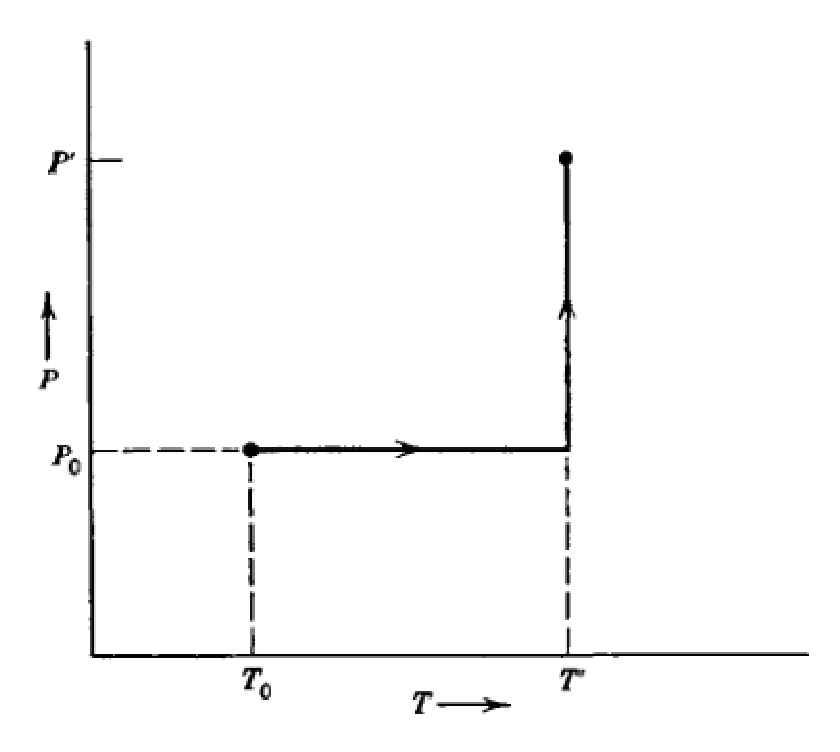
\includegraphics[scale=0.7]{fig3_9.eps}
}
\end{example}

\subsection*{习题}
